\section{Auswertung}
\label{sec:Auswertung}

\subsection{Bestimmung von $C_p$ und $C_V$}
\label{sec:C_p-C_V}

Zunächst wird die Molwärme bei konstantem Druck $C_p$ bestimmt. $C_p$ kann wie folgt bestimmt werden:

\begin{equation}
    C_p = \frac{U \cdot I \cdot M \cdot \increment t}{m \cdot \increment T}
    \label{eq:C_p}
\end{equation}

$U$ und $I$ sind hierbei die angelegte Heizspannung und Heizstrom der Probe für den jeweiligen Zeitraum zwischen 2 Messwerten, $M$ ist die Molmasse des Materials der Probe, $m$ ist die Masse der Probe, $\increment T$ ist die Temperaturdifferenz, die zwischen 2 Messwerten auftritt und $\increment t$ ist die Zeitdifferenz zwischen 2 Messwerten. Die Molmasse $M$ und die Masse $m$ der Probe beträgt:

\begin{align*}
    M &= 0, \! 06355 \, \frac{\mathrm{kg}}{\mathrm{mol}} \\
    m &= 0, \! 342 \, \mathrm{kg}
\end{align*}

Um die gemessenen Pt-100-Widerstände in die entsprechenden Temperaturen umzurechnen kann folgende Formel genutzt werden:

\begin{equation}
    T = 0, \! 00134 \, R^2 + 2, \! 296 R - 243, \! 02
\end{equation}

Für $R$ wird der Widerstand in Ohm eingesetzt und die sich daraus ergebende Temperatur $T$ besitzt die Einheit °C. Anschließend wird die Temperatur von der Probe $T_P$ und dem Zylinder $T_Z$ gemittelt und mit der gemittleten Temperatur $T$ wird im Folgenden gerechnet. 

Aus $C_p$ lässt sich mit Formel \eqref{eq:C_V} $C_V$ bestimmen:

\begin{equation}
    C_p - C_V = 9 \cdot \alpha^2 \cdot \kappa \cdot V_0 \cdot T \, \, \, \, \, \, \Leftrightarrow \, \, \, \, \, \, C_V = C_p - 9 \cdot \alpha^2 \cdot \kappa \cdot V_0 \cdot T
    \label{eq:C_V}
\end{equation}

$\alpha$ ist dabei der lineare Ausdehnungskoeffizient, $\kappa$ \cite{kappa} ist das Kompressionsmodul und $V_0$ \cite{V0} ist das Molvolumen. Für Kupfer können folgende Werte für $\kappa$ und $V_0$ verwendet werden:

\begin{align*}
    \kappa &= 140 \, \mathrm{GPa} \\
    V_0 &= 7, \! 11 \cdot 10^{-6} \, \frac{\mathrm{m}^3}{\mathrm{mol}}
\end{align*}

Die Werte von $\alpha$ sind nicht konstant sondern abhängig von der Temperatur der Probe, deswegen wird eine Ausgleichsrechnung mit einem Polyonom 4. Grades

\begin{equation}
    \alpha (T) = a \cdot T^4 + b \cdot T^3 + c \cdot T^2 + d \cdot T + e
    \label{eq:alpha}
\end{equation}

durch die Werte aus Abbildung \ref{fig:alpha} durchgeführt.

\begin{figure}
    \centering
    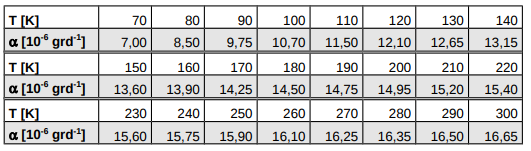
\includegraphics[width=0.8\textwidth]{build/alpha.PNG}
    \caption{$\alpha$ für verschiedene Temperaturen $T$. \cite{Anleitung}}
    \label{fig:alpha}
\end{figure}

Diese Ausgleichsrechnung wird mit Python und $scipy.optimize.curve\_fit$ erstellt und die Unsicherheiten mit $uncertainties.ufloat$ berechnet. Dies ergab folgende Werte für die Parameter

\begin{align*}
    a &= (-8, \! 2 \pm 0, \! 7) \cdot 10^{-9} \, \mathrm{K}^{-5} \\
    b &= (7, \! 4 \pm 0, \! 5) \cdot 10^{-6} \, \mathrm{K}^{-4} \\
    c &= (2, \! 5 \pm 0, \! 1) \cdot 10^{-3} \, \mathrm{K}^{-3} \\
    d &= (0, \! 41 \pm 0, \! 02) \, \mathrm{K}^{-2} \\
    e &= (11, \! 3 \pm 0, \! 6) \, \mathrm{K}^{-1}
\end{align*}

und folgenden Plot:

\begin{figure}[H]
    \centering
    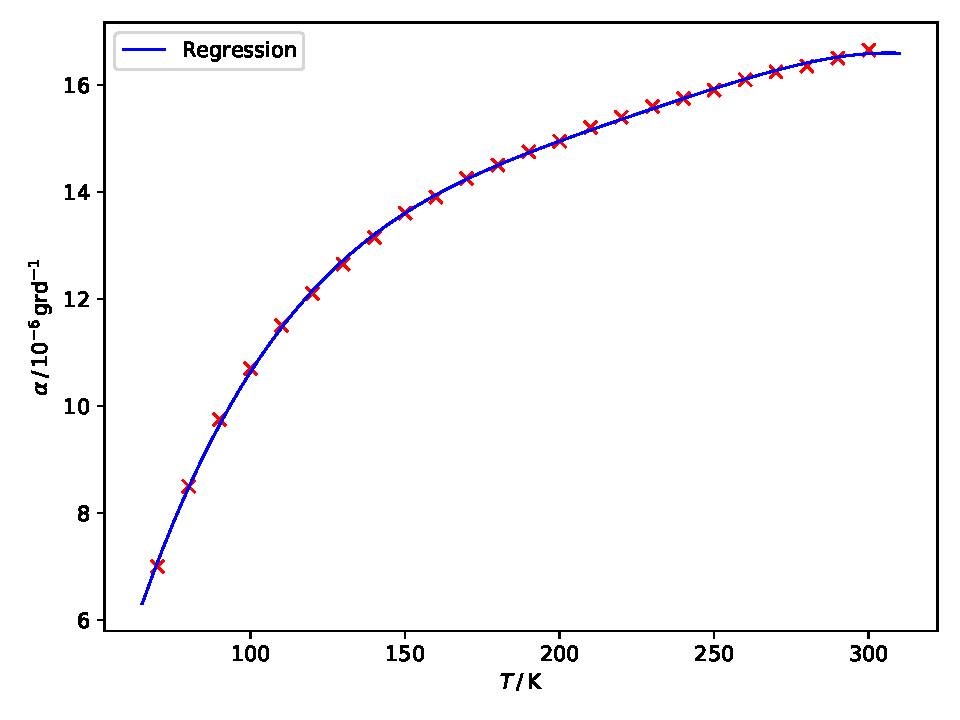
\includegraphics[width=0.8\textwidth]{build/alpha.pdf}
    \caption{$\alpha$ in Abhängigkeit von $T$ mit Ausgleichsrechnung.}
    \label{fig:alpha_plot}
\end{figure}

Mit Hilfe von dieser Ausgleichsfunktion in Abbildung \ref{fig:alpha_plot} kann $C_V$ in Abhängigkeit von der Temperatur $T$ mit Formel \eqref{eq:C_V} berechnet werden. Die Werte für $C_p$ und $C_V$ sind in Tabelle \ref{tab:C} zu sehen.

%Tabelle einfügen mit R_P, R_Z, T_P, T_Z, T, t, U, I, C_p, C_V und \label{tab:C} hier einfügen
\begin{table}
    \centering
    \caption{Messdaten und Berechnungen für Bestimmung von $C_p$ und $C_V$. }
    \csvreader[tabular = c c c c c c c c|c c,
    head=true,
    table head=$t \:/\: \si{\minute}$ & $R_P\:/\: \si{\kilo\ohm}$ &  $R_Z \:/\: \si{\kilo\ohm}$ &$T_P \:/\: \si{\milli\ampere}$ &$T_Z \:/\: \si{\milli\ampere}$ & $ \langle T\rangle \:/\: \si{\milli\ampere}$ &$ U \:/\: \si{\volt}$ & $I \:/\: \si{\milli\ampere}$ & $C_P$&$C_V$\\ \midrule,
    late after line= \\]
    {datendat-copy.csv}{}{\csvcoli & \csvcolii & \csvcoliii & \csvcoliv& \csvcolv& \csvcolvi& \csvcolvii & \csvcolviii & \csvcolix & \csvcolx}
    \label{tab:C}
\end{table}
Diese Werte in einem Diagramm aufgetragen gegen die Temperatur $T$ ergibt:

\begin{figure}[H]
    \centering
    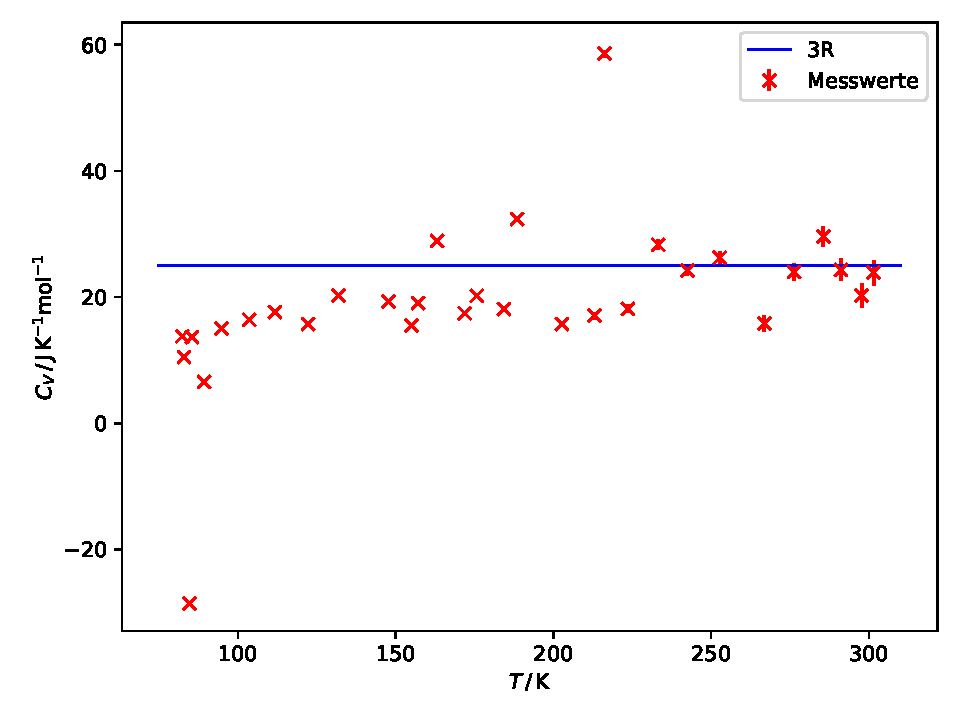
\includegraphics[width=0.8\textwidth]{build/C_V.pdf}
    \caption{$C_V$ in Abhängigkeit von $T$ mit Fehlerbalken.}
    \label{fig:C_V}
\end{figure}

In Abbildung \ref{fig:C_V} ist zu erkennen, dass es bei der Messung einige Messfehler aufgetreten sind. Deswegen werden die Werte Nummer 4, 5 und 21 aus Tabelle \ref{tab:C} als Messfehler herausgenommen und erneut in einem Diagramm gegen die Temperatur $T$ aufgetragen.

\begin{figure}[H]
    \centering
    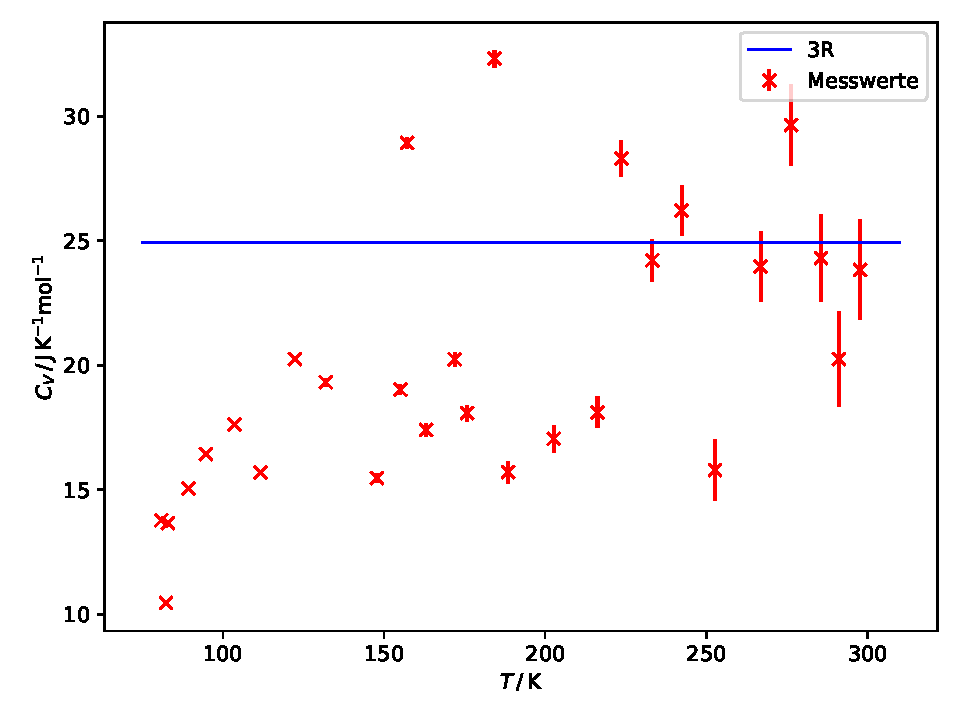
\includegraphics[width=0.8\textwidth]{build/C_V_gefiltert.pdf}
    \caption{$C_V$ in Abhängigkeit von $T$ mit Fehlerbalken.}
    \label{fig:C_V_gefiltert}
\end{figure}

In den folgenden Abschnitten wird auch nur mit den Werten von $C_V$ aus Abbildung \ref{fig:C_V_gefiltert} gerechnet.

\subsection[Experimentelle Bestimmung der Debye-Temperatur]{Experimentelle Bestimmung der Debye-Temperatur $\theta_D$}
\label{sec:debye_temp}

Zur Bestimmung der Debye Temperatur $\theta_D$ werden nur die Molwärmen $C_V$ für eine Temperatur von unter $170 \, \mathrm{K}$ betrachtet. Mit Hilfe der Debye-Funktion aus Quelle \cite{Anleitung} können die Werte für $\frac{\theta_D}{T}$ für die entsprechenden $C_V$ bestimmt werden. $\frac{\theta_D}{T}$ multipliziert mit der entsprechenden Temperatur $T$ ergibt dann die Debye Temperatur $\theta_D$. Die Werte für $T$, $C_V$, $\frac{\theta_D}{T}$ und $\theta_D$ sind in Tabelle \ref{tab:Debye} aufgetragen.

%Tabelle mit T, C_V, theta_D/T, theta_D und \label{tab:Debye} hier einfügen
\begin{table}
    \centering
    \caption{Messdaten zur Berechnungen von $\theta_D$.}
    \csvreader[tabular = c c c c,
    head=true,
    table head=$C_V \:/\: \si{\joule\per\kelvin\per\mole}$ & $T \:/\: \si{\kelvin} $ &  $\frac{\theta_D}{T}$ & $\theta \:/\: \si{\kelvin}$\\ \midrule,
    late after line= \\]
    {C_v_und_T-copy.csv}{}{\csvcoli & \csvcolii & \csvcoliii & \csvcoliv}
    \label{tab:Debye}
\end{table}

Die verschiedenen Werte für die Debye-Temperatur $\theta_D$ ergeben gemittelt:

\begin{equation*}
    \theta_D = (329 \pm 19) \, \mathrm{K}
    \label{eq:debye}
\end{equation*}

Der Mittelwertsfehler wurde mit Formel \eqref{eq:mittel} bestimmt.

\begin{equation}
    \sigma_{\overline{x}} = \frac{\sigma}{\sqrt{n}} = \sqrt{\frac{1}{n^2 - n} \cdot \sum\limits_{i=1}^{n} \left( \, \overline{x} - x_i \right)^2}
    \label{eq:mittel}
\end{equation}

Dabei ist $\sigma_{\overline{x}}$ der Mittelwertsfehler, $n$ ist die Anzahl der Werte über die gemittelt wird und $\overline{x}$ ist der Mittelwert.

\begin{figure}[H]
    \centering
    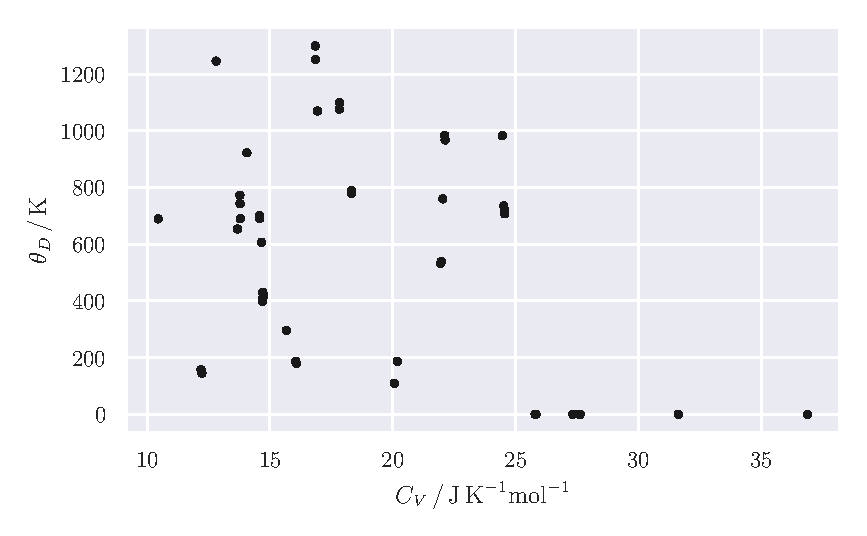
\includegraphics[width=0.7\textwidth]{build/Theta_C_V.pdf}
    \caption{$\theta_D$ in Abhängigkeit von $C_V$.}
    \label{fig:Theta_C_V}
\end{figure}

\begin{figure}[H]
    \centering
    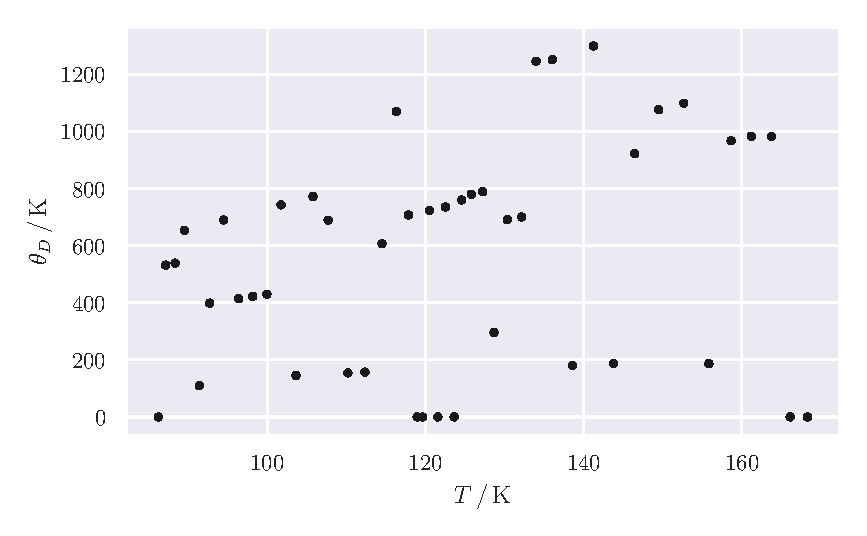
\includegraphics[width=0.7\textwidth]{build/Theta_T.pdf}
    \caption{$\theta_D$ in Abhängigkeit von $T$.}
    \label{fig:Theta_T}
\end{figure}

\subsection[Theoretische Bestimmung der Debye-Temperatur]{Theoretische Bestimmung der Debye-Temperatur $\theta_D$}
\label{sec:theo_debye_temp}

Die Debye Temperatur kann auch theoretisch bestimmt werden. Dazu wird Formel \eqref{eqn:udebye} aus Abschnitt \ref{sec:debye} verwendet. Für die Geschwindigkeiten $v_l$ und $v_{tr}$ werden die Werte aus Quelle \cite{Anleitung} genutzt, diese lauten:

\begin{align*}
    v_l &=  4, \! 7 \, \frac{\mathrm{km}}{\mathrm{s}} \\
    v_{tr} &= 2, \! 26 \, \frac{\mathrm{km}}{\mathrm{s}}
\end{align*}

Mit Hilfe von Formel \eqref{eqn:Z} ergibt sich dann mit den Geschwindigkeiten $v_l$ und $v_{tr}$ für die Debye-Frequenz $\omega_D$ folgende Formel:

\begin{equation}
    \omega_D = \sqrt[3]{\frac{18 \pi^2 N_A}{V_0} \cdot \left( \frac{1}{v_l^3} + \frac{2}{v_{tr}^3} \right)^{-1} }
    \label{eq:omega}
\end{equation}

$N_A = 6, \! 022 \cdot 10^ {23} \, \mathrm{mol}^{-1}$ ist dabei die Avogadro-Konstante. Die Werte eingesetzt ergibt dann für die Debye-Frequenz folgenden Wert:

\begin{equation*}
    \omega_D = 4, \! 349 \cdot 10^{13} \, \mathrm{Hz}
\end{equation*}

Die Debye-Temperatur $\theta_D$ lässt sich nun mit Formel \eqref{eq:debye-temp} bestimmen.

\begin{equation}
    \theta_D = \frac{\hbar}{k_B} \cdot \omega_D
    \label{eq:debye-temp}
\end{equation}

Dabei ist $\hbar = 1, \! 055 \cdot 10^{-34} \, \mathrm{Js}$ \cite{h_quer} das reduzierte planksche Wirkungsquantum und $k_B = 1, \! 381 \cdot 10^{-23} \, \frac{\mathrm{J}}{\mathrm{K}}$ \cite{k_B} ist die Boltzmann-Konstante. Damit ergibt sich für die Debye-Temperatur $\theta_D$ ein theoretischer Wert von:

\begin{equation*}
    \theta_D = 332, \! 102 \, \mathrm{K}
\end{equation*}
